\chapter{Implementierung und Tests}

Ebenfalls Teil der Resultate dieser Arbeit sind die Implementierung und die Tests der entwickelten Systeme.
In den erwarteten Resultaten wurde formuliert, dass die Implementierung als Bestandteil der Arbeit einfach zugänglich und ausführbar sein soll.

Nach der Erarbeitung der Resultate aus der Korrelation und der Klassifikation folgt die Entwicklung des Systems, welches die topologischen Indizes sinnvoll vergleicht.

Eine Übersicht über den Ablauf der Applikation ist in Abbildung \ref{fig:flowchart} zu sehen.

\begin{figure}[H]
    \centering
    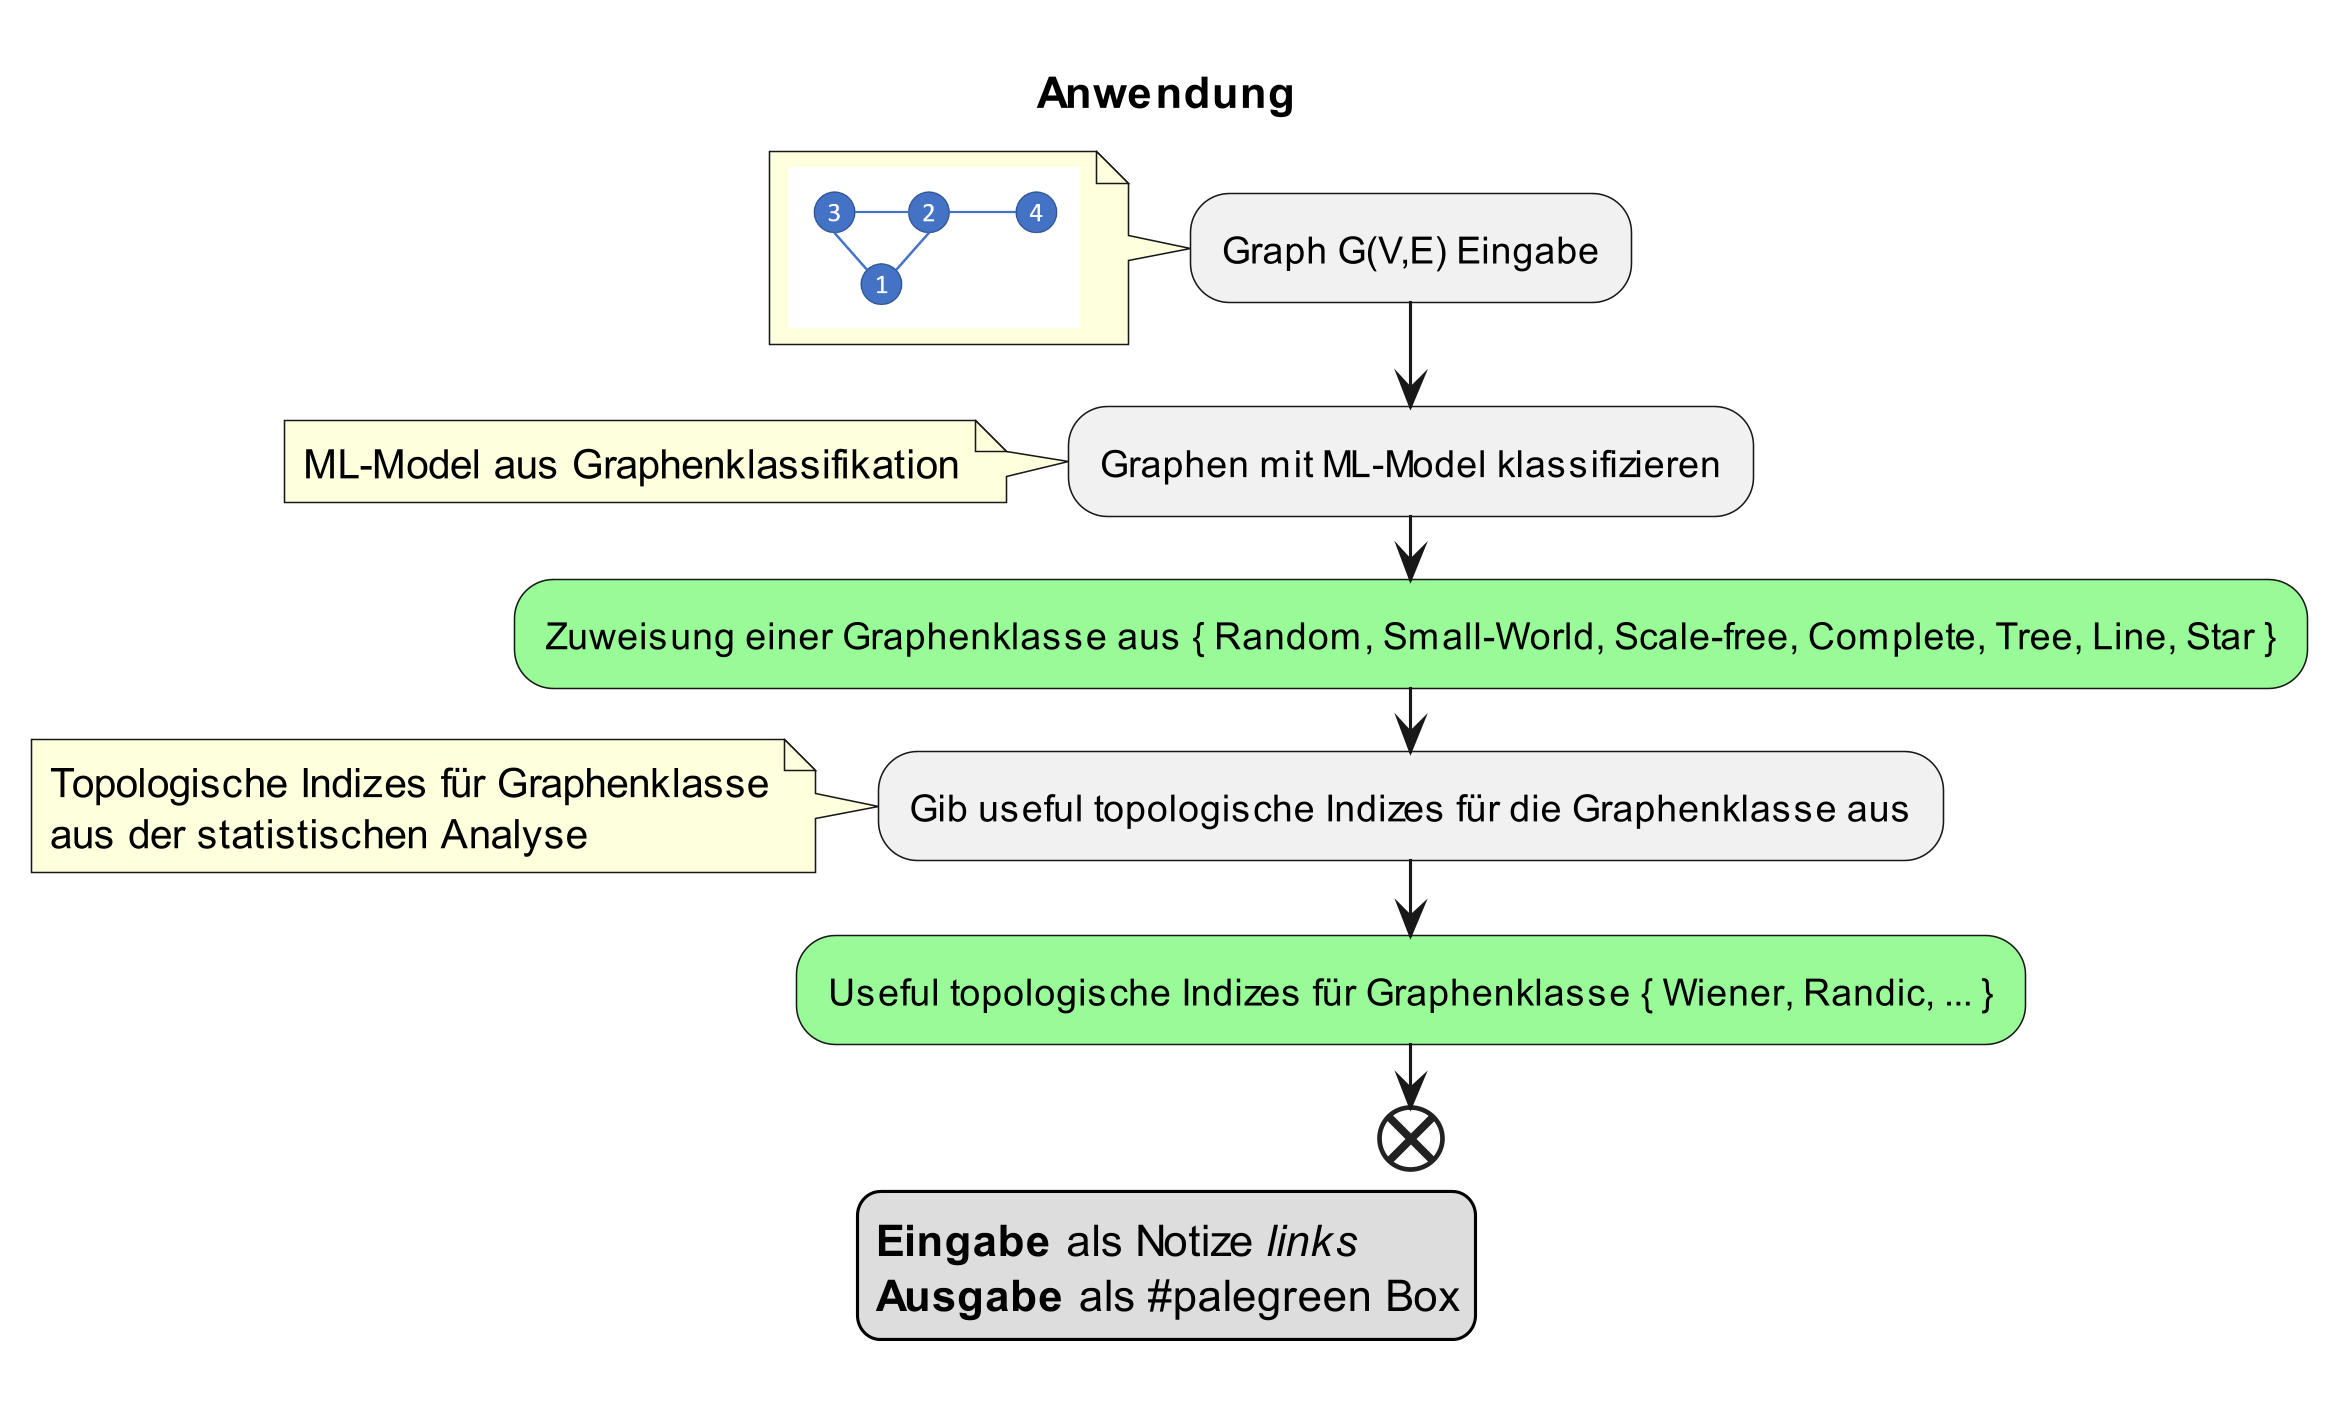
\includegraphics[width=0.7\textwidth]{images/30_results/activity_app.png}
    \caption{Ablauf der Anwendung für die Berechnung der nützlichen topologischen Indizes für ein Netzwerk}
    \label{fig:flowchart}
\end{figure}

\newpage

\section{Die Entwicklungsumgebung}

\subsection{Gründe für den Einsatz von Python}

Die Programmiersprache Python wird in dieser Recherche für die Netzwerkanalyse eingesetzt, obwohl auch die Programmiersprache R eine Vielzahl an Paketen für diese Aufgabe bereitstellt.

Allerdings ist Python auf GitHub weiterverbreitet als R.
Ein wesentlicher Vorteil von Python im Vergleich zu R, besteht in der Nutzung von Jupyter-Notebooks, welche die Entwicklung und Dokumentation der Netzwerkanalyse erleichtern.
Durch die Kombination von Experimenten, Daten und Ergebnissen in einem Dokument können Letztere effektiv präsentiert werden.
Matplotlib wird verwendet, um die Ergebnisse in Diagrammen darzustellen.

\subsection{NetworkX}

NetworkX ist die bekannteste und am meisten verwendete Bibliothek für die Netzwerkanalyse in Python \cite{hagberg_exploring_2008}.
Die Anwendung ist simpel und die Dokumentation weit fortgeschritten.

Ein Beispiel für das Erstellen eines einfachen Graphen mit NetworkX ist:

\begin{listing}[H]
    \begin{minted}[frame=lines,framesep=2mm,baselinestretch=1.2,bgcolor=LightGray,fontsize=\footnotesize,linenos]{python3}
import networkx as nx

G = nx.Graph()
G.add_node(1)
G.add_nodes_from([2, 3])
G.add_edge(1, 2)
G.add_edges_from([(1, 2), (1, 3)])
    \end{minted}
    \caption{Erstellen eines einfachen Graphen mit NetworkX}
\end{listing}

\subsection{GrinPy}

GrinPy ist eine Bibliothek für die Netzwerkanalyse in Python \cite{amos_grinpy_2022}, die auf die Analyse von Graphen mit Attributen spezialisiert ist.
Die Dokumentation ist noch nicht weit fortgeschritten.

GrinPy ist eine Erweiterung von \mintinline{python3}{NetworkX} und besitzt eine Vielzahl an Funktionen, um topologische Indizes von Graphen zu berechnen.
Somit können topologische Indizes von Graphen, welche durch NetworkX erstellt wurden, direkt berechnet werden. Die Graphen müssen nicht erst in ein anderes Format konvertiert werden.

\subsection{Matplotlib}

Matplotlib ist eine Bibliothek für die Visualisierung von Daten in Python \cite{Hunter:2007} und wird eingesetzt, um die Ergebnisse der Netzwerkanalyse in Diagrammen darzustellen.
Dies ist für die explorative Datenanalyse und das Verständnis der Ergebnisse nützlich.

Auch kann die Bibliothek verwendet werden, um die Ergebnisse in einem Dokument zu visualisieren.
Die Integration in die Skripts und Jupyter-Notebooks ist unkompliziert. Ergebnisse können direkt ausgegeben und betrachtet werden.
Zudem können die Bilder auch in verschiedenen Formaten zur weiteren Bearbeitung abgespeichert werden.

\subsection{PyTorch Geometric}

PyTorch Geometric \cite{fey_lenssen_2019} ist eine Graph-Machine-Learning-Bibliothek, welche eine Erweiterung von PyTorch \cite{Paszke_PyTorch_An_Imperative_2019} entwickelt darstellt.
Sie ist entwickelt worden, um schnell und einfach Graph Neural Networks zu implementieren.
Sie kann für verschiedene Anwendungen eingesetzt werden, unter anderem für \textbf{Node-Level-Predictions}, \textbf{Edge-Level-Predictions} oder in diesem Fall \textbf{Graph-Level-Predictions}.

Die Bibliothek ist optimal dokumentiert und bietet eine Vielzahl an Beispielen, welche die Implementierung von Graph Neural Networks erleichtern.

\subsection{Pandas}

Pandas ist eine Bibliothek für die Datenanalyse in Python \cite{mckinney-proc-scipy-2010}.
Im Kontext der Arbeit eignet sich Pandas besonders, um die berechneten topologischen Indizes in einem Data-Frame zu speichern.
Wie bereits in Code-Listing \ref{lst:indices} beschrieben, wird als Index der Tabelle jeweils der Name (Index) des Graphen verwendet.
Die Spalten des Data-Frames sind die verschiedenen Werte der topologischen Indizes.

Diverse statistische Methoden sind direkt in Pandas implementiert. 
Unter anderem können die Mittelwerte, Standardabweichungen und Mediane direkt berechnet werden. 
Aber auch die Korrelation zwischen den jeweiligen topologischen Indizes kann vereinfacht angezeigt und ausgegeben werden.


\section{Applikation und Code}

Es folgt der Code zur Entwicklung eines Python-Moduls, welches die Berechnung der nützlichen topologischen Indizes in verschiedenen Graphenklassen ermöglicht.
Das Modul kann auf GitLab unter \url{https://git.ffhs.ch/luca.hostettler/bt-hostettler} gefunden werden.

Es ist in zwei Schritte unterteilt:
\begin{enumerate}[itemsep=0pt]
    \item \textbf{Eingabe eines Graphen,}
    \item \textbf{Empfehlungen der topologischen Messwerte}
\end{enumerate}

\subsection{Eingabe des Graphen}

Das Programm akzeptiert als Eingabe einen NetworkX-Graphen.
Aus der Datenanalyse wurde die Usefulness einzelner topologischer Indizes für verschiedene Netzwerkarten ermittelt. Dabei wurden die Netzwerke in folgende Kategorien eingeteilt: \textbf{Random}, \textbf{Small-World}, \textbf{Scale-free}, \textbf{Complete}, \textbf{Line}, \textbf{Tree} und \textbf{Star}. Die Klassifizierung des Graphen erfolgt mit dem GCN-Modell aus Abschnitt \ref{sec:classification}, welches bereits beschrieben und trainiert wurde.

\begin{listing}[H]
    \begin{minted}[frame=lines,framesep=2mm,baselinestretch=1.2,bgcolor=LightGray,fontsize=\scriptsize,linenos]{python}    
# create an instance of the app
app = App()
# create a sample graph using networkx
graph = nx.path_graph(150)
# test graph classification
g_class = app.classify(graph)

print(f"Found graph class {app.class_keys[g_class]}")
# get the topological indices
topological_indices = app.get_topological_indices(graph)
# print the topological indices
print(topological_indices)
    \end{minted}
    \caption{Code zum Einlesen des Graphen}
\end{listing}

Wie im vorhergehenden Code-Listing ersichtlich, ist der benötigte Code für die Applikation überaus kurz und einfach. Dabei ist \mintinline{python3}{App} die Klasse, welche die Applikation implementiert. Die Methode \mintinline{python3}{classify} ist für die Klassifikation des Graphen zuständig. Die Methode \mintinline{python3}{get_topological_indices} ist für das Laden und Anzeigen der für den Graphen nützlichen topologischen Indizes verantwortlich.

\subsection{Das GCN-Modell}

Das Rezept für das Modell besteht aus in drei Schritten:

\begin{enumerate}
    \item jeden Knoten mit Node-Embedding verarbeiten,
    \item alle Node-Embeddings in ein gemeinsames Graph-Embedding zusammenfassen (ReadOut-Layer) und
    \item die Klassifizierung auf Graph-Embedding trainieren.
\end{enumerate}

\begin{listing}[H]
    \begin{minted}
        [frame=lines,framesep=2mm,baselinestretch=1.2,bgcolor=LightGray,fontsize=\footnotesize,linenos]
        {python}    
class GCN(torch.nn.Module):
    def __init__(self, hidden_channels=64, num_node_features=3, num_classes=7):
        super(GCN, self).__init__()
        torch.manual_seed(12345)
        self.conv1 = GCNConv(num_node_features, hidden_channels)
        self.conv2 = GCNConv(hidden_channels, hidden_channels)
        self.conv3 = GCNConv(hidden_channels, hidden_channels)
        self.lin = Linear(hidden_channels, num_classes)

    def forward(self, x, edge_index, batch):
        # 1. Obtain node embeddings
        x = self.conv1(x, edge_index)
        x = x.relu()
        x = self.conv2(x, edge_index)
        x = x.relu()
        x = self.conv3(x, edge_index)

        # 2. Readout layer
        x = global_mean_pool(x, batch)  # [batch_size, hidden_channels]

        # 3. Apply a final classifier
        x = F.dropout(x, p=0.5, training=self.training)
        x = self.lin(x)

        return x
    \end{minted}
    \caption{Der Code für das GCN-Modell}
    \label{lst:code_gcn}
\end{listing}

\subsection{Code für die Klassifikation des Graphen}

Das oben aufgeführte Modell \ref{lst:code_gcn} wird verwendet, um die Klassifikation des Graphen zu bestimmen.
Diese wird in zwei Schritten durchgeführt:

\begin{enumerate}
    \item \textbf{Aufbereitung der Eingabe}
    \item \textbf{Klassifikation des Graphen}
\end{enumerate}

\begin{listing}[H]
    \begin{minted}
        [frame=lines,framesep=2mm,baselinestretch=1.2,bgcolor=LightGray,fontsize=\footnotesize,linenos]
        {python}    
# classify the graph
def classify(self, G):
    node_labels = np.arange(G.number_of_nodes())
    degrees = nx.degree_centrality(G)
    betweenness = nx.betweenness_centrality(G)
    attrs = dict(zip(node_labels, node_labels))
    nx.set_node_attributes(G, attrs, "label")
    nx.set_node_attributes(G, degrees, "degree")
    nx.set_node_attributes(G, betweenness, "betweenness")
    # convert to torch tensor
    x = from_networkx(graph, group_node_attrs=["label", "betweenness", "degree"])
    test_loader = DataLoader([x], batch_size=1, shuffle=False)
    # run the model
    for x in test_loader:
        out = self.model(x, x.edge_index, x.batch)
        # convert to numpy
        pred = out.argmax(dim=1)  # Use the class with highest probability
        # return the result
        return pred
    \end{minted}
    \caption{Code zur Klassifikation des Graphen}
\end{listing}

\subsection{Empfehlungen der topologischen Messwerte}

In der Konsole werden, zusammen mit der vorhergesagten Klasse des Graphen, die vorgeschlagenen topologischen Indizes ausgegeben.

\begin{listing}[H]
    \begin{minted}
        [frame=lines,framesep=2mm,baselinestretch=1.2,bgcolor=LightGray,fontsize=\footnotesize,linenos]
        {python}    
# get the topological indices
def get_topological_indices(self, graph):
    # classify the graph
    y = self.classify(graph)
    # get the topological indices
    topological_indices = y[0]
    # return the topological indices
    return topological_indices
    \end{minted}
    \caption{Code für den Vorschlag der topologischen Indizes}
\end{listing}

In einem späteren Schritt wird zusammen mit den vorgeschlagenen topologischen Indizes eine Erklärung geliefert.

Die Idee ist, dass die Erklärung zur \textit{Explainability} beiträgt. 
Als Kontext sind zwei Punkte relevant: zum einen die topologischen Indizes, welche vorgeschlagen werden, und zum anderen die vorhergesagte Klasse des Graphen.
